\chapter{Unsupervised Learning}
whiUnsupervised learning works by observing data distribution ${\bf P}_data$,  while lacking a target variable.\\
There are several applications to this: \\
{\bf DIMENSIONALITY REDUCTION}, find a function f that maps each input $x \in \mathscr{X}$ to a lower dimensional embedding, where dim($\mathscr{Y}$) $ < $ dim($\mathscr{X}$). \\
Why would one want to do this? By compressing the input data we also reduce the feature dimensionality making the input more lightweight thus reducing the time for data elaboration.\\
{\bf CLUSTERING} finds a function $f$ that assigns each input $x \in \mathscr{X}$ to a cluster. Why? \\
It allows to analyze data by grouping it together and can also be used to compress data with similar patterns.\\
{\bf DENSITY ESTIMATION} find a probability distribution $f \in \triangle \mathscr{X}$ that fits the data $x \in \mathscr{X}$. Why? 
Allows for explicit estimate of an unknown probability distribution, generating new data and detecting anomalies.\\
\section{Principal component analysis}
The main idea is to fidn the direction of maximum variance, change the coordinate system and then dropping dimensions of least variance. \\
\begin{definition}[Variance and Covariance]
	Measure of the spread of a set of points around their center of mass (the mean)
\end{definition}

I don't really know how to explain easily eigenvalues and eigenvectors so I'm just gonna put a picture of the example.
\\
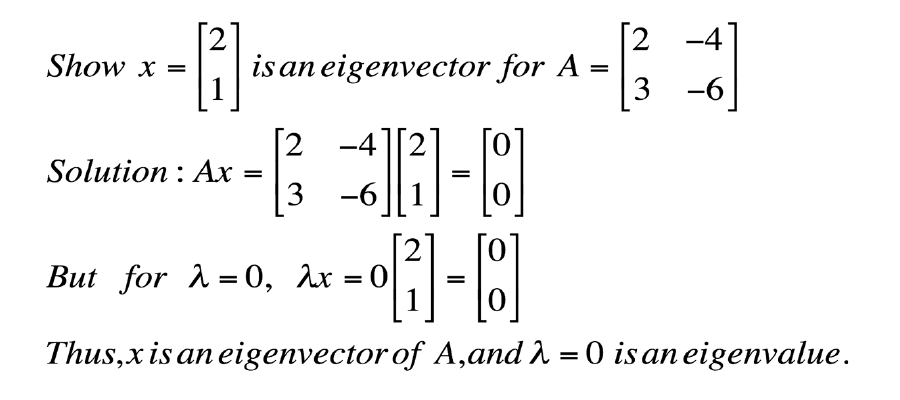
\includegraphics[scale=0.5]{eigen}

It can be shown that the largest eigenvalue is the variance along the first principal component.

\section{Clustering}
The goal is to divide data into clusters. What K-means clustering does is fix a number of k clusters and divides the data with the least amount of variance inside the clusters.
\[
min \sum_{j=1}^{k}V(\mathscr{C})
\]
Some properties are that it is sensitive to the scale of features, it is guaranteed to converge although it's not guaranteed to find a global minimum. \\
The problem with K-means clustering is that it requires spherical clusters. It is also a {\bf hard cluster}, meaning that example belong exactly to one cluster only. \\
{\bf EM-Clustering } (Expectations Maximization) on the other hand is a soft clustering technique that takes data as a mixture of gaussian.

With EM clustering you start with initial cluster centers, you soft assign points to each cluster and then iterate.\\
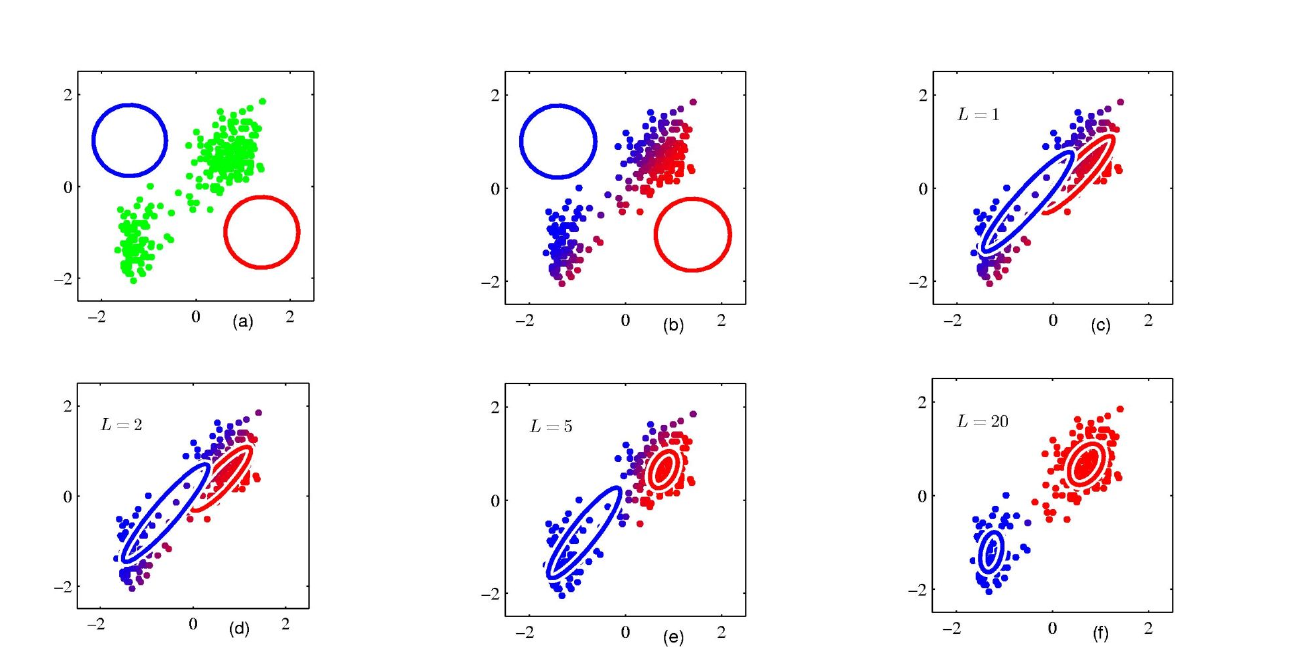
\includegraphics[scale=0.3]{em}
To recalculate the centers we need them to fit a gaussian.

There are other means of clustering namely spectral clustering (using graphs), hierarchical graphs, agglomerative clustering etc.